\section{Анализ требований к программному средству и разработка функциональных требований}
\label{sec:domain}

\subsection{Варианты использования программного средства}
\label{sec:domain:use_cases}

По результатам анализа предметной области и существующих аналогов можно сделать вывод, что проектируемое программное средство должно поддерживать ряд функций для автоматизации некоторых процессов учёта персонального бюджета, ключевыми из которых являются следующие:

\begin{itemize}
    \item \emph{Поддержка множественных валют}.
    Возможность учитывать расходы и доходы в различных приносит большую гибкость и повышает удобство пользования приложением.
    \item \emph{Управление счетами}, которое позволяет полностью манипулировать существующими источниками средств пользователя.
    \item \emph{Отображение списка счетов}, позволяющее наглядно видеть расположение и количество текущих денежных средств.
    \item \emph{Сводные значения по счетам}.
    Возможность отображения общей суммы по всем валютам и количества денег, которое можно потратить до следующей зарплаты, являются крайне полезной информацией для контроля личных денежных средств и избавления от лишних трат.
    \item \emph{Управление категориями} доходов и расходов, которые помогают распределить денежные траты для последующего анализа и оптимизации расходов.
    \item \emph{Просмотр статистики по категориям} позволит определить наиболее затратные категории расходов и узнать, куда конкретно уходят деньги.
    \item \emph{Управление транзакциями}.
    Функция является основной в проектируемом программном средстве и позволяет регистрировать все операции с деньгами в системе.
    \item \emph{Отображение списка транзакций по дням} позволяет использовать просматривать и работать с существующими транзакциями.
\end{itemize}

Диаграмма вариантов использования, разработанная с использованием нотации \uml, представлена на рисунке~\ref{fig:domain:use_cases:model}.

\begin{figure}
    \centering
    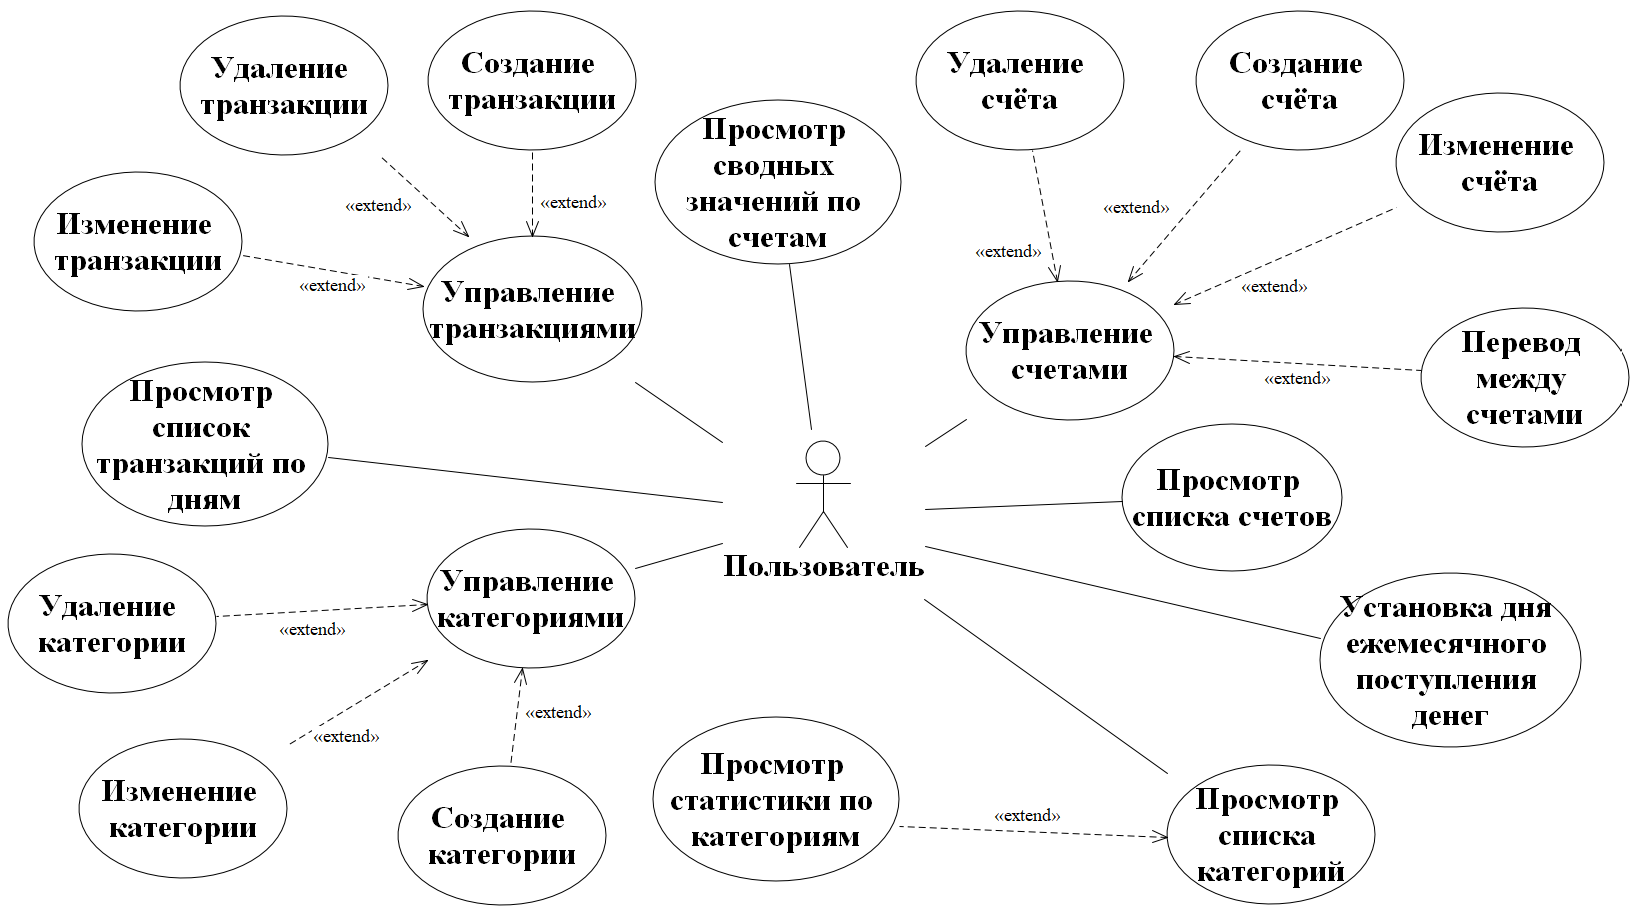
\includegraphics[scale=0.37]{2_1_use_case_model.png}
    \caption{Диаграмма вариантов использования ПС}
    \label{fig:domain:use_cases:model}
\end{figure}

Из диаграммы видно, что основные функции программного средства, а именно управление счетами, транзакциями и категориями, состоят из основных операций работы с данными, такими как создание, изменение и удаление соответствующего объекта.
Вместе с просмотром различных списков сущностей программного средства, данные варианты использования обеспечивают пользователю возможности по учёту доходов и расходов, описанные в подразделе~\ref{sec:analysis:literature:tracking}.

\emph{Просмотр статистики по категориям} позволяет пользователю оптимизировать расходы, обращая внимание на самые затратные категории расходов.

\emph{Сводные значения по счетам} могут быть использованы как основа для реализации любого из методов планирования бюджета, описанного в подразделе~\ref{sec:analysis:literature:planning}.

\subsection{Разработка инфологической модели базы данных}
\label{sec:domain:db}

Концептуальное (инфологическое) проектирование — построение семантической модели предметной области, то есть информационной модели наиболее высокого уровня абстракции.
Такая модель создается без ориентации на какую-либо конкретную СУБД и модель данных.
Основными конструктивными элементами инфологических моделей являются сущности, связи между ними и их свойства (атрибуты).

Исходя из необходимости использования в проектируемом приложении базы данных, разработаем ее инфологическую модель.
Для ее создания будем использовать расширение диаграммы классов \uml, предназначенное для моделирования баз данных.
Полученная диаграмма (рисунок~\ref{fig:domain:db:model}) будет являться моделью базы данных инфологического уровня~\cite{kulikov_db_workbook}.

\begin{figure}
    \centering
    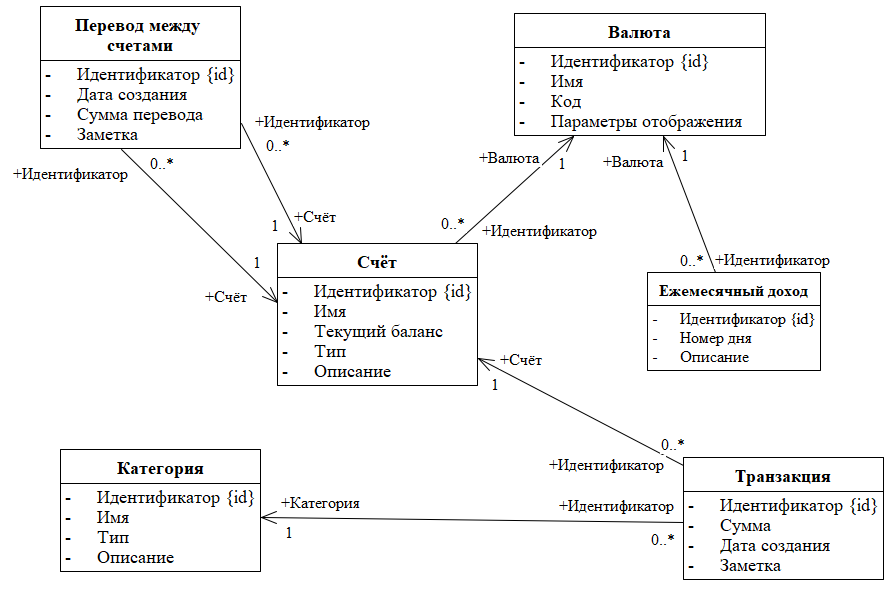
\includegraphics[scale=0.70]{2_2_logical_model.png}
    \caption{Инфологическая модель базы данных ПС}
    \label{fig:domain:db:model}
\end{figure}

Одной из особенностей разработанной модели является отсутствие сущности <<Пользователь>>.
Исходя из того, что под результатом дипломного проектирования предполагается \emph{однопользовательское} программное средство, разворачиваемое на мобильном устройстве -- ПС не нуждается в сохранении дополнительной информации о пользователе.
Однако, в будущем планируется ввести возможности по синхронизации данных с удаленным сервером.
При таком случае данные о пользователе, а именно данные аутентификации и авторизации, можно будет сохранить в локальном хранилище приложения.

Далее рассматривается отдельно каждую из сущностей, представленной на диаграмме.

Сущность <<Валюта>> содержит информацию о денежных единицах, которая позволяет совершать пользователю работать с несколькими валютами одновременно.
Предполагается, что атрибут <<Код>> должен представляться в общепринятом трёхсимвольном коде валюты по стандарту ISO~4217~\cite{iso_4217}.
Атрибут <<Параметры отображения>> необходим для того, чтобы отображать конкретные денежные значения в общепринятом и знакомом для каждой валюты формате. Например, суммы в долларах США обычно записываются в виде <<\$100>>, а суммы в белорусских рублях -- <<100 руб.>>.

Сущность <<Счёт>> содержит актуальную информацию об пользовательском хранилище денежных средств.
<<Тип>> счета позволяет указать на то, является ли он сберегательным или нет.
Эта информация вносит больше гибкости в процесс планирования расходов и актуальна в момент расчета лимита расходов на день с учетом даты следующего поступления денег.
Данная сущность находится в связи с сущностью <<Валюта>>, так как каждый счёт хранит денежные средства той валюты, с которой связан.

Сущность <<Категория>> представляет собой отдельное направление расходов или доходов пользователя.
Атрибут <<Тип>> определяет вид транзакций, связанных с данной категорией и определяет, был совершен \emph{доход} или \emph{расход}.

Сущность <<Транзакция>> является основной в проектируемом ПС и определяет разовую операцию с денежными средствами.
Экземпляры сущности содержат в себе информацию о размере денежных средств, участвующих в операции, а также дату совершения операции.
<<Транзакция>> связана с сущностью <<Категория>>, благодаря чему можно определить, является ли конкретная транзакция расходом или доходом.
Также она связана с сущностью <<Счёт>>, что определяет валюту, в которой была проведена операция.

Сущность <<Перевод между счетами>> содержит информацию о переносе денежных средств между двумя счетами проектируемого программного средства.
Данная сущность имеет две связи с сущностью <<Счёт>>, определяя, откуда и куда была перемещена сумма денег сумму денег.

Сущность <<Ежемесячный доход>> представляет данные о дате ожидаемого поступления денег и позволяет оценить количество денег, которые можно ежедневно тратить до такого поступления.
<<Ежемесячный доход>> связан с сущностью <<Валюта>>, так как расчёт лимита денег на день предполагается рассчитывать среди денег этой же валюты.

\subsection{Разработка спецификации функциональных требований}
\label{sec:domain:specification}

На основе поставленных целей, задач и требований, определённых в подразделе~\ref{sec:analysis:specification}, а также разработанной функциональной модели программного средства учёта персонального бюджета, возможно представить детализацию функций проектируемого ПС.

\subsubsection{} Поддержка множественных валют
\label{sec:domain:specification:currencies}

При реализации функции поддержки множественных валют должны быть учтены следующие требования:

\begin{enumerate}
    \item доступ к списку всех существующих валют;
    \item конечный список валют заблаговременно определен;
    \item коды валют соответствуют стандарту ISO~4217;
    \item запись денежных сумм осуществляется с учётом особенностей каждой валюты.
\end{enumerate}


\subsubsection{} Функция управления счетами
\label{sec:domain:specification:wallets}

Функция управления счетами должна быть реализована с учетом следующих требований:

\begin{enumerate}
    \item У пользователя должна быть возможность создания счёта.
    \item Пользователь должен иметь возможность изменить любой существующий счёт.
    \item Изменение баланса счёта не должно влиять на другие сущности.
    \item Должна быть возможность удаления счёта.
    \item При удалении счёта все связанные с ним транзакции должны быть также удалены.
    \item Должна присутствовать возможность денежного перевода с одного счёта на другой с изменением соответствующих значений балансов счетов.
    \item При денежном переводе необходимо учитывать возможное различие валют счетов.
\end{enumerate}

\subsubsection{} Функция отображения списка счетов
\label{sec:domain:specification:wallets_list}

Реализация функции отображения списка счетов должна учитывать следующие требования:

\begin{enumerate}
    \item Должна предоставляться возможность выбора сортировки элементов списка среди следующих:
    \begin{enumerate}
        \item алфавитный порядок по имени счёта;
        \item по порядку создания -- наиболее ранние сверху;
        \item по порядку создания -- наиболее поздние сверху.
    \end{enumerate}
    \item Элементы списка должны содержать следующую информацию о счёте:
    \begin{enumerate}
        \item имя;
        \item тип (повседневный или сберегательный);
        \item текущий баланс;
        \item валюта.
    \end{enumerate}
    \item Список должен обновляться при любых операциях с транзакциями и счетами.
\end{enumerate}

\subsubsection{} Функция отображения сводных значений по счетам
\label{sec:domain:specification:wallets_stats}

При отображении сводных значений по счетам должны быть учтены перечисленные требования:

\begin{enumerate}
    \item Должен быть произведен расчёт и отображение общего баланса всех счетов, сгруппированных валютам.
    \item Пользователь должен иметь возможность просматривать количества денег в день по каждой валюте, в которых он указал ежемесячное поступление денег.
    \begin{enumerate}
        \item При этом сумма должна рассчитываться в зависимости от ближайшего по времени дня поступления средств по каждой валюте.
        \item Счета сберегательного типа не должны участвовать в расчёте данного показателя.
    \end{enumerate}
    \item Сводные значения должны обновляться после любых операций счетами и транзакциями.
\end{enumerate}

\subsubsection{} Функция управления категориями
\label{sec:domain:specification:categories}

При разработке данной функции необходимо учитывать:

\begin{enumerate}
    \item Возможность создания категории.
    \item При создании.
    \item Возможность удаления категории, при которой пользователь должен иметь возможность выбрать одну из двух опций:
    \begin{enumerate}
        \item удалить все связанные с этой категорией транзакции;
        \item переместить все связанные с этой категорией транзакции на другую существующую категорию.
    \end{enumerate}
    \item В ПС должны присутствовать по одной стандартной категории доходов и расходов, которые представляют собой значение <<Без категории>>.
    \item Пользователь не должен иметь возможности удалить стандартную категорию.
\end{enumerate}

\subsubsection{} Функция отображения статистики по категориям.
\label{sec:domain:specification:categories_stats}

При реализации функции отображения множественных валют должны быть учтены следующие требования:

\begin{enumerate}
    \item Статистика по категориям должна отображаться в виде списков всех категорий.
    \item Списки категорий различных типов (доходов и расходов) должны отображаться раздельно.
    \item Должен быть выбор периода расчёта статистики и валюты, по которой производится подсчёт.
    \item Должна предоставляться возможность выбора сортировки элементов списка среди следующих:
    \begin{enumerate}
        \item алфавитный порядок по имени категории;
        \item по убыванию общей суммы всех транзакций по данной категории;
        \item по порядку создания -- наиболее ранние сверху;
        \item по порядку создания -- наиболее поздние сверху.
    \end{enumerate}
    \item Элементы списка должны содержать следующую информацию с учётом заданных валюты и периода времени:
    \begin{enumerate}
        \item имя категории;
        \item количество транзакций, совершенных для данной категории;
        \item общая сумма всех транзакций, совершенных для данной категории;
        \item процентное содержание суммы всех транзакций, совершенных для данной категории, относительно других категорий.
    \end{enumerate}
    \item Статистика по категориям должна обновляться при любых операциях с транзакциями или категориями.
\end{enumerate}

\subsubsection{} Функция управление транзакциями
\label{sec:domain:specification:transactions}

Реализация функции управления транзакциями должна учитывать следующие требования:

\begin{enumerate}
    \item Должна присутствовать возможность создания транзакции.
    \item Пользователь должен иметь возможность изменять любые значения всех существующих транзакций.
    \item У пользователя должна быть возможность удаления любой транзакции.
    \item При любых операциях с транзакциями должны изменяться соответствующие значения балансов связанных с ними счетов.
\end{enumerate}

\subsubsection{} Функция отображения списка транзакций по дням
\label{sec:domain:specification:transactions_list}

При реализация функции отображения транзакций необходимо принимать во внимание следующие требования:

\begin{enumerate}
    \item Список транзакций должен представляться в виде двухуровневого списка, отсортированного в порядке убывания дат совершения транзакции:
    \begin{enumerate}
        \item Каждый элемент внешнего списка должен представлять собой один календарный день.
        \item Внутренние списки должны содержать в себе все транзакции, совершенные в соответствующий календарный день.
        \item Элемент внутреннего списка должен представлять собой одну транзакцию.
    \end{enumerate}
    \item Для каждой транзакции должна быть отображена следующая информация:
    \begin{enumerate}
        \item сумма транзакции с учётом записи определённой валюты;
        \item имя счёта, связанного с данной транзакцией;
        \item имя категории, в которую была совершена транзакция;
        \item тип транзакции (доход или расход).
    \end{enumerate}
    \item У пользователя должна быть возможность просматривать информацию о сумме всех транзакций по каждому дню.
    \item Список должен обновляться при любых операциях с транзакциями.
\end{enumerate}
